\capitulo{3}{Conceptos teóricos}

En este apartado se desarrollarán los conceptos teóricos necesarios para la comprensión total del proyecto. Se explicarán desde conceptos generales, hasta conceptos más específicos de las tecnologías empleadas.

Para entender el contexto de este proyecto, primero es necesario definir que es la gestión de tareas, así como todos los conceptos teóricos ligados a ellas.

\section{Gestión de tareas}
La gestión de tareas se define como un sistema estratégico y dinámico diseñado para la planificación y ejecución de tareas de forma eficaz, garantizando que la trayectoria de las mismas se lleve a cabo de forma ágil hasta su finalización. Cuando se trata de rutinas diarias, las tareas se completan en diversas fases, en las cuales se definen enfoques únicos. La dominancia de estas fases y la adaptación de la estrategia es la llave para desbloquear la productividad eficiente y el cumplimiento de los plazos establecidos.

Este concepto se puede confundir con la gestión de proyectos, la diferencia entre ambos se define en: la gestión de tareas se centra en la tareas individuales orientadas al ámbito profesional y laboral. Mientras que en la gestión de proyectos se centra en la ejecución exclusiva de objetivos profesionales. 
\subsection{Fases de la gestión de tareas}
La gestión de tareas es un sistema que necesita de cuatro fases para ejecutarse de forma eficaz:

\begin{itemize}
    \item \textbf{Etapa inicial:} se crea la tarea y se definen los objetivos de la misma.
    \item \textbf{Segunda fase:} se asigna a un responsable para llevar a cabo la tarea.
    \item \textbf{Tercera fase:} el responsable avanza con la realización de la tarea.
    \item \textbf{Cuarta fase:} se realiza una supervisión y control de la calidad de la tarea realizada.
\end{itemize}

Las tareas propuestas pueden ser eliminadas una vez se cumplan con los objetivos establecidos o también pueden ser abandonadas en caso de que los objetivos ya no sean necesarios. Además, la realización de las tareas se pueden realizar de forma conjunta o individual.

\subsection{Pautas para ser eficiente en la gestión de tareas}

Para lograr una gestión eficaz es necesario comprender todos los conceptos y herramientas, y emplearlas en el plan que se vaya a acometer. Se pueden emplear distintos pasos para lograrlo:

\begin{itemize}
    \item En el caso de la tarea requiera de un equipo de trabajo, el plan se deberá de ajustar a los objetivos del equipo.
    \item Dedicar el tiempo necesario a cada tarea, estableciendo prioridades y realizando ajustes de tiempo.
    \item Priorizar la organización de las tareas, lo que ahorrará confusiones y centrará el trabajo en lo importante.
    \item Realizar un seguimiento de los progresos alcanzados a lo largo de las fases de la tarea. Esto ayudará a localizar que tarea requiere más atención.
\end{itemize}

\subsection{Pasos clave en la gestión de tareas}

La gestión de tareas requiere de algunos pasos críticos que actúan como papel vital en su funcionamiento.

\begin{itemize}
    \item \textbf{Priorización:} es importante diferenciar la importancia de las tareas, una buena definición de prioridades permite que los plazos de entrega se completen con total eficacia. Unas buenas prácticas de priorización permiten reservar tiempo para la realización de otras tareas.
    \item \textbf{Seguimiento:} realizar un seguimiento de los objetivos y progresos de las tareas es vital para detectar la ausencia de componentes de gestión, es decir, lo que falta y lo que se necesita para la próxima tarea.
    \item \textbf{Programación:} este paso es muy importante, ya que permite definir las temporalidades de ejecución de las tareas y cuando deben de ser completadas para obtener los mejores resultados. Además, permite establecer un calendario robusto sobre el que trabajar.
\end{itemize}

\subsection{Perfiles que hacen uso de la gestión de tareas}
Cuando se trata de gestión de tareas, no existen restricciones de quien puede hacer uso de ello. Sin embargo, es recomendable que lo usen aquellos que tengan una agenda apretada y requieran de una organización rápida y eficaz. Los perfiles personas que más recurren a la gestión de tareas son:

\begin{itemize}
    \item \textbf{Jefes de equipo:} desde jefe de proyectos hasta altos cargos de empresas. Generalmente, su agenda suele estar cargada con muchas tareas y a veces suelen colapsarse unas con otras. La gestión de tareas facilita la realización de tareas a tiempo.
    \item \textbf{Equipos de trabajo:} los equipos de trabajo se caracterizan por tener que realizar muchas tareas, repartidas entre los distintos miembros. Por ello, la gestión de tareas permite distribuir el trabajo a realizar entre los miembros, con el fin de agilizar el proceso de ejecución de las tareas.
    \item \textbf{Gestión personal:} permite a un individuo gestionar sus propias tareas que pueden ser: educativas, domésticas o profesionales. Con ello, se logra minimizar las perdidas de tiempo.
\end{itemize}

\subsection{Ventajas de la gestión de tareas}
\begin{itemize}
    \item \textbf{Productividad:} la gestión de tareas potencia la productividad, ya que elimina tareas que son innecesarias de la rutina cotidiana. 
    \item \textbf{Eficiencia:} cada tarea tendrá a su disposición los recursos necesarios para ser completada sin contratiempos. Además, la claridad en la organización de tareas, acelera el proceso de toma de decisiones.
    \item \textbf{Gestión del tiempo:} el hecho de planificar los acontecimientos con antelación previene perdidas de tiempo innecesarias. Por otro lado, el tiempo sobrante puede ser empleado para la realización de otras tareas.
    \item \textbf{Toma de decisiones:} al dividir el trabajo en distintas tareas, facilita la toma de decisiones sobre las prioridades o tiempos de estas, dando una visión más amplia sobre las labores a realizar.
    \item \textbf{Reducción del estrés:} cuando se ha realizado la asignación de todas las tareas, se reduce el estrés de haber olvidado alguna tarea de vital importancia.
    
\end{itemize}

\subsection{Herramientas de gestión de tareas}

Para poder llevar a cabo una buena gestión de tareas es necesario hacer uso de distintas herramientas que nos ayuden a tener una mejor visión del trabajo que hay que completar.

\begin{itemize}
    \item \textbf{Lista de tareas pendientes:} las tareas se estructuran en un listado que permite hacer una vista rápida de lo que hay que hacer.
    \item \textbf{Tableros:} las tareas se distribuyen de forma que se puedan distinguir por prioridades y ayudan a los usuarios a visualizarlas.
    \item \textbf{Diagramas:} sirven para representar gráficamente las tareas. Un ejemplo claro es el diagrama de Gantt, también usado en este proyecto. Este permite representar mediante líneas la fecha de inicio y fin de una tarea, así como la duración de la misma. Esto permite tener una visión clara de como se puede distribuir el tiempo para ejecutar las tareas de la forma más eficiente.
    \item \textbf{Calendarios:} los calendarios ayudan a ubicar las fechas de las tareas, así como a permiten añadir recordatorios o plazos personalizados.
\end{itemize}

\subsection{Técnicas de gestión de tareas}
\begin{itemize}
    \item \textbf{Descartar tareas menos importantes:} aquellas tareas que no sean de vital importancia, deberán de ser descartadas para priorizar las más importantes. Una vez se ejecuten las de mayor importancia, se podrá destinar el tiempo restante a otras labores.
    \item \textbf{Evitar multitarea:} la realización de múltiples tareas supone que el esfuerzo será la mitad, además se producirán perdidas de tiempo. Lo aconsejable es centrarse en la realización de un tarea y completarlas de una en una \cite{gestion_tareas}.
\end{itemize}

\section{Diagrama de Gantt}
Un diagrama de Gantt es una herramienta gráfica que permite representar el tiempo o duración de distintas tareas a lo largo del tiempo.

El formato más común de diagrama se basa en la enumeración de tareas de forma vertical de izquierda a derecha. Se establecen dos puntos, el comienzo de la tarea y el fin de la misma. Entre ambos puntos se traza una linea horizontal que representa la duración de cada tarea.

El diagrama de Gantt permite revisar las tareas pendientes de hacer, cuándo se esperan realizar o como dependen unas de otras.

En 1896 el ingeniero polaco, Karol Adamiecki, creó el armonograma (predecesor del diagrama de Gantt). Años más tarde, el ingeniero y consultor estadounidense, Henry Gantt, desarrolló su propia versión que unificaba a ambos gráficos, con el fin de evaluar la productividad de su fábrica \cite{gantt_wikipedia}.

\subsection{Componentes de un diagrama de Gantt}
Un diagrama de Gantt de forma simple se compone de una lista de tareas, una línea de tiempo horizontal y barras horizontales que representan las tareas a realizar. Todos los componentes que lo componen son:

\begin{itemize}
    \item \textbf{Lista de tareas:} lista vertical de las tareas a realizar.
    \item \textbf{Linea de tiempo:} linea horizontal que muestra los días, semanas o meses en las que transcurren las tareas.
    \item \textbf{Bares:} marcadores horizontales que representan a las tareas con su duración y fechas de inicio y fin.
    \item \textbf{Fecha:} línea vertical que representa la fecha actual.
\end{itemize}

\subsection{Cuándo utilizar un diagrama de Gantt}
Se debe de hacer uso de un diagrama de Gantt cunado se requiera de la visualización de las tareas a realizar. Permite tener una visión centrada en el tiempo del trabajo que se debe de realizar. También, da una visión de las siguientes tareas a la realización de otras.

Un diagrama de Gantt es útil en los siguientes casos:
\begin{itemize}
    \item \textbf{Planificación de tareas:} cuando se quieren visualizar todas las tareas, incluso las más pequeñas.
    \item \textbf{Programación de tareas:} cuando se quiere ver la duración de las tareas y cuando se finalizarán por completo.
\end{itemize}

\subsection{Ventajas e inconvenientes de los diagramas de Gantt}

El uso de este tipo de diagramas implica ciertas ventajas, pero también algunos inconvenientes. Las ventajas de su uso son:
\begin{itemize}
    \item Representación clara de las tareas del proyecto, indicación de plazos, etc.
    \item Facilidad para compartir con las partes implicadas en las tareas
\end{itemize}

Algunos de los inconvenientes que presenta son:
\begin{itemize}
    \item Cuando existen muchas tareas, pueden ser más compleja la creación de un diagrama de Gantt.
    \item Se debe de disponer de todas las fechas de las tareas para que puedan ser representadas \cite{gantt_canva}.
\end{itemize}


\section{API}
El término \textit{API} hace referencia a \textit{Application Programming Interfaces}, es decir, interfaz de programación de aplicaciones. Consiste en un conjunto de definiciones y protocolos que se utilizan para integrar el software de las aplicaciones, permitiendo la comunicación entre dos aplicaciones software mediante un conjunto de reglas. Podemos entender una \textit{API} como un puente que facilita el intercambio de información y funcionalidades entre dos aplicaciones distintas \cite{api_xataka}.

\subsection{Objetivo de una API}
El objetivo principal de una \textit{API} es facilitar el trabajo a los desarrolladores, además de tiempo y dinero. Por ejemplo, se puede implementar un servicio de pago sin la necesidad de integrar un servicio de pago desde cero.

\subsection{Funcionamiento de una API clientes-servidor}
La arquitectura de las \textit{API} se basa en el modelo \textit{cliente-servidor}. La aplicación que envía una solicitud se denomina cliente, y la que envía la respuesta se denomina servidor. Las \textit{API} pueden funcionar de cuatro formas diferentes \cite{api_amazon}:

\begin{itemize}
    \item \textbf{API de SOAP:} utiliza el protocolo simple de acceso a datos. El cliente y el servidor intercambian mensajes a través de \textit{XML}.
    
    \item \textbf{API de RPC:} se denominan llamadas a procedimientos remotos. El cliente completa un procedimiento en el servidor, y el servidor retorna el resultado al cliente.
    
    \item \textbf{API de WebSocket:} esta \textit{API} utiliza objetos \textit{JSON} para transmitir datos. Una ventaja de estas es la comunicación bidireccional entre aplicaciones cliente y el servidor. El servidor tiene la capacidad de enviar mensajes de devolución de llamada a los clientes.
    
    \item \textbf{API de REST:} en esta \textit{API} el cliente envía las solicitudes al servidor como datos. El servidor hace uso de la entrada del cliente para inicializar las funciones internas y retorna los datos de salida del cliente.
    REST hace referencia a la transferencia de estado representacional. En esta se definen un conjunto de funciones como \textit{GET, PUT, POST, DELETE, etc}. que los clientes pueden hacer uso de para acceder a los datos que se encuentren alojados en el servidor. Todos estos datos son intercambiados mediante \textit{HTTP}.
\end{itemize}

\begin{figure}[H]
    \centering
    {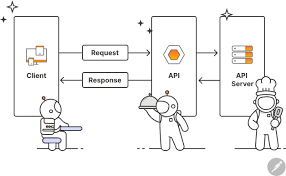
\includegraphics[width=0.7\linewidth]{img/funcionamiento_api.png}}
     {\caption{Esquema del funcionamiento de una API}
     \label{fig:funcionamiento_api}}
\end{figure}

\section{APK}
Los archivos con extensión \textit{.apk} son ejecutables diseñados para el sistema móvil \textit{Android}, este término se refiere a \textit{Android Application Package}. Se utiliza para distribuir e instalar aplicaciones en dispositivos que hagan uso del sistema operativo Google \cite{apk_xataka}.
La creación de los archivos \textit{APK} transcurre en dos fases:
\begin{itemize}
    \item Compilación de un programa para \textit{Android}.
    \item Empaquetamiento de todas sus partes en un solo archivo.
\end{itemize}
Posteriormente el archivo \textit{APK} contendrá todo el código, recursos, activos, certificados y archivo \textit{manifest}.

Los distintos componentes de un archivo \textit{APK} son \cite{apk_browserstack}\cite{apk_wikipedia}:
\begin{itemize}
    \item \textbf{AndroidManifest.xml:} archivo de manifiesto adicional que define el nombre, versión, permisos requeridos, actividades y servicios que utiliza , versiones compatibles de Android y otros metadatos necesarios.
    \item \textbf{assets:} directorio que contiene archivos que pueden ser accedidos por la aplicación en tiempo de ejecución, estos pueden ser \textit{archivos de configuración, fuentes, HTML o multimedia}. Estos archivos deben de ser accedidos a través de AssetManager.
    \item \textbf{classes.dex:} clases compiladas en el formato de archivo dex, legibles por la máquina virtual Dalvik.
    \item \textbf{lib:} contiene bibliotecas nativas compiladas y que son especificas de una capa de software de procesador. Son empleadas cuando la aplicación de depende de código en C o C++ requerido para operaciones críticas de rendimiento.
    \item \textbf{META-INF:} almacena el certificado, la firma, y un archivo manifiesto de la aplicación, empleado para verificar la integridad y autenticidad de la \textit{APK}.
    \item \textbf{res:} directorio que contiene recursos sin compilar, como pueden ser archivos XML, imágenes, iconos y componentes de interfaz de usuario.
    \item \textbf{resources.arsc:} archivo que contiene recursos precompilados, permite que la aplicación cargue contenido relacionado con el idioma.
\end{itemize}

\section{Desarrollo multiplataforma}
El desarrollo multiplataforma consiste en la codificación de aplicaciones que pueden ser ejecutadas en distintos sistemas operativos o plataformas. Cada sistema operativo o plataforma, de forma habitual, requiere de un lenguaje de programación en concreto para la creación de software. Esto se debe a que cada sistema hace uso de una interfaz de programación de aplicaciones propia, es decir, el conjunto de instrucciones que indican como debe de interactuar el software con el sistema \cite{multiplataforma}.

El desarrollo multiplataforma minimiza el proceso de crear una versión software específica para cada sistema operativo, esto se logra usando un lenguaje que pueda funcionar con diferentes interfaces de programación de aplicaciones. Por ello, con la codificación de un solo código fuente se puede crear un software ejecutable en distintos sistemas.

\subsection{¿Cuáles son los beneficios del desarrollo multiplataforma?}
El desarrollo multiplataforma brinda múltiples beneficios a aquellos programadores que recurren a su uso. Estos beneficios son:
\begin{itemize}
    \item Mayor alcance de usuario en el mercado.
    \item Reducción de costes de producción.
    \item Aumento de la reutilización de código.
\end{itemize}

\section{Persistencia}
La persistencia hace referencia a la propiedad de los datos por la cual estos permanecen sin llegar a desaparecer. Si se hace referencia a este término en programación, indica la acción de mantener la información de un objeto de forma permanente y que puede ser recuperada en cualquier momento.
Los datos pueden tener una duración efímera, lo que quiere decir que en el momento en el que estos cambian su valor ya no hay persistencia.

\subsection{Tipos de persistencia}
\subsubsection{Persistencia de aplicación}
Capacidad mediante la cual los datos sobreviven a la ejecución del programa que los ha creado. Sin esta capacidad, los datos desaparecen en cuanto el equipo se queda sin energía, ya que estos residirían en la memoria RAM, y esta es volátil. Por ello, es necesario que los datos se almacenen en un medio de almacenamiento secundario, que no pierda los datos en cuanto se quede sin energía. Por ejemplo, se puede guardar en disco un fichero con la configuración de un programa para que el usuario no tenga que volver a configurarlo la próxima vez que lo ejecute.

\subsubsection{Persistencia de objetos}
La persistencia de objetos se basa en la inicialización de objetos con sus atributos \cite{persistencia}. Esto se logra de dos formas:
\begin{itemize}
    \item Un medio de almacenamiento fijo guarda un conjunto de datos que son recuperados cuando el tipo de objeto es creado, posteriormente esos datos se traspasan a las propiedades del objeto creado.
    \item Un objeto almacena los datos que serán transferidos al nuevo objeto cuando sea creado. Por lo tanto, los datos están almacenados en memoria.
\end{itemize}

Para almacenar los datos en un medio físico se recurre a un mecanismo llamada serialización, que contiene en una secuencia de bytes todos los datos del objeto.

La persistencia, en el ámbito de programación, permite almacenar, transferir y recuperar el estado de los objetos. Existen varias formas de hacerlo:
\begin{itemize}
    \item Serialización.
    \item Mapeo relacional de objetos.
    \item Bases de datos orientadas a objetos.
\end{itemize}

\section{Programación asíncrona}
La programación asíncrona permite evitar retrasos durante la ejecución de un programa. Cuando las ejecuciones son síncronas se pueden producir bloqueos durante la ejecución debido a la necesidad de esperar a que se ejecute algún proceso, lo que puede provocar un bloqueo total del programa hasta que termine de ejecutarse dicho proceso \cite{asincrona_softplan}.

Las operaciones asíncronas más comunes son \cite{asincrona_dart}:
\begin{itemize}
    \item Obtención de datos de la red.
    \item Escritura de datos en una base de datos.
    \item Lectura de datos de un archivo.
\end{itemize}

Las principales ventajas del uso de programación asíncrona son:
\begin{itemize}
    \item Permite la ejecución de múltiples tareas, garantizando que no se van a producir bloqueos.
    \item Evita el bloqueo de interfaces por la ejecución de operaciones largas.
\end{itemize}
